\documentclass[11pt, twocolumn]{article}
\usepackage[T1]{fontenc}
\usepackage{amsmath, amssymb}
\usepackage{mathtools}
\usepackage{graphicx}
\usepackage[utf8]{inputenc}
\usepackage{fdsymbol}
\usepackage{textgreek}
\usepackage{natbib}
\usepackage{hyperref}
\usepackage{nameref}
\usepackage{url}
\usepackage{array}
\usepackage{csquotes}
\usepackage{caption}
\usepackage{algpseudocode}
\usepackage[toc,page]{appendix}
\DeclarePairedDelimiter\floor{\lfloor}{\rfloor}
\providecommand{\myceil}[1]{\left \lceil #1 \right \rceil }
\hypersetup{
    colorlinks,
    citecolor=black,
    filecolor=black,
    linkcolor=black,
    urlcolor=black
}

\title{Decentralized state machine using Nakamoto (probabilistic) consensus\\\medskip Research Project 2022}
\author{Nicolas COURAUD (nicolas.couraud@etu.emse.fr)\\École Nationale Supérieure des Mines de Saint-Étienne}

\begin{document}

\maketitle
\onecolumn
\section*{Abstract}

As defined by Schneider \cite{stateMachine}, the state machine approach is a general method for implementing a fault-tolerant service
by replicating servers and coordinating client interactions with server replicas.

In this article, we look at state machines as a way to hold in multiple servers copies of the same record. That record, in my implementation, is a standard
key-value data structure (\href{https://go.dev/blog/maps}{a Go map}).

I show how one can build a decentralized state machine using Nakamoto Consensus (in our implementation we used the Snowball consensus algorithm), and I study the advantages
and drawbacks of such an approach, compared to classical consensus algorithms like Raft \cite{understandable}.

The implementation of the project is available at \href{https://github.com/Nicolascrd/distributed-state-machine}{github.com/Nicolascrd/distributed-state-machine}


\tableofcontents

\section{Traditional state machine replication}

\subsection{Introduction}

Decentralized state machine systems are currently built, for the most part, around classical consensus algorithms.

In classical consensus, all of the nodes have to know each other. It is a permissioned model, which means that nodes have to get an approval to get into the network.
That is very normal for private infrastructure but might not work for public infrastructure. Because all nodes must communicate with each other, the communication cost in generally considered high.

Many classical consensus algorithms exists, the most famous one being Paxos \cite{parliament}. In my project, I used the Raft consensus algorithm \cite{understandable} because it has the same performances
as Paxos, and is simpler to understand and implement.

In Raft, each node can be either Leader, Follower or Candidate. In regular functioning, one node will be the leader and all the others will follow.
The Leader node sends regular heartbeat requests to notify followers that it is still running. If they stop receiving the heartbeat, they switch to the follower status.

The client can ask any node to add a log to the record.
The request includes the number of the log that the client wants to add and the log himself. If the client as a node which is not the leader, the request is transfered to the leader. If there is already a record at that number,
the leader returns an error message to the client. Otherwise, the leader updates its record and asks all his followers to update themselves as well.

When requesting a log, the client can also query any node in the network. The node just responds with the log at that number in the local record that it is holding.

The only parameter than I included in my implementation is \emph{updateSystem}, which is a boolean. If True, if the leader sends heartbeats and a node does not reply, it will be eliminated from the network in the knowledge of all the nodes. This make it possible to
crash a majority of nodes and still have the state machine running and usable on all the surviving nodes.

\subsection{Byzantine fault-tolerance (BFT) with classical consensus}

Contrary to Crash Fault, Byzantine Fault \cite{byzantine} is a type of failure where you consider that the node can fail in any possible way. In practice, it means that the node will stay up and can send malicious requests to
interfere with the functioning of the network.

My implementation of the state machine does not tolerate Byzantine Faults at all. With only one byzantine node, it already endangers the whole system. Indeed, the malicious node can "elect himself" in Raft, and then send heartbeats to all
the node in the network, including the legitimate leader to become the leader de facto. Then, it can ignore requests, reply whatever it wants and write any log it wants in any node it wants.

To tackle this issue, BFT algorithms were designed (such as \cite{pbft}). They include a layer of authentification, but are not necessarily much slower. However, there is a maximum number of malicious nodes that the algorithm can handle safely \cite{partialSynchrony}.
For example, assuming partial synchrony of the nodes, consensus protocols can handle t crash failures with 2t+1 nodes but t byzantine failures with no less than 3t+1 nodes.

\section{Nakamoto (probabilistic) state machine replication}
\subsection{The Nakamoto Consensus}

Nakamoto consensus was introduced with the bitcoin blockchain \cite{bitcoin}. Nakamoto consensus is probabilistic, which means that there is a probability ε that consensus is not reached.
Of course, ε can be so low that crucial systems can be built relying Nakamoto consensus. Nakamoto consensus is open : nodes don't have to register or get an authorisation to enter the network.
Because nodes don't have to know every other node in the network and be able to communicate with everyone, Nakamoto is supposed to allow for greater scale in the network.

Nakamoto consensus definetly shaked the consensus space in computer science with cryptocurrencies. In a different context, can it be useful as well ?

\subsection{My Nakamoto state machine implementation}

To implement Nakamoto consensus, I chose the Snowball consensus algorithm \cite{snowprotocol}, which underlies the Avalanche blockchain.

The goal of snowball is to reach binary consensus starting from a network of nodes.

I adapted the protocol to fit the needs of a decentralized state machine, because snowball is described in the context of building a payment system (because it is the basis of Avalanche, which is that payment system).
Snowball is built by iterations, but I will only focus on Snowball, the last iteration, because it is the most interesting and the one I tested the performances in the end. Slush and Snowflake are interesting to understand
where we are coming from, but no more.

I adapted Snowball in the following ways : Each node, in addition to having all the snowball consensus related data (not much), has a version of the record. All nodes starts with a empty record.
Because it is the requirement for a decentralized state machine, each node can be queried to add a log to the record. Each node can also be queried to get one log in the record.

The snowball protocol is triggered when the client asks to add a new log to an index that has not been touched yet. Indeed, the system works as if each index in the record corresponds to an independant snowball run.

In snowball, each node has a counter of "confidence" which can tip towards one way or another. In my implementation, there is no binary consensus because the only value the system has is the log request.
When receiving an add-log request, the node follows this sequence :
\begin{algorithmic}
    \State from request (client or other node):
    \State $logToAdd$ (string)
    \State $logPosition$ (int)

    \State \\from node memory :
    \State $record$ (map[int]string)
    \State $cnt$ (map[int]int)
    \\
    \If{$record[logPosition]$ exists}
    \State reply $record[logPosition] == logToAdd$
    \Else
    \State $record[logPosition] \gets logToAdd$
    \State reply $True$
    \State initiateRequest($logToAdd$, $logPosition$)
    \EndIf

\end{algorithmic}

initiateRequest corresponds to the following sequence :

\begin{algorithmic}
    \While{$True$}
    \State $success \gets initiateQuery(req)$
    \State $initiateQuery$ picks a sample in the network and queries it
    \If{$success$}
    \State $cnt[logPosition]++$
    \Else
    \If{$cnt[logPosition] == 1$}
    \State delete($record$, $logPosition$)
    \State $cnt[logPosition] \gets 0$
    \Else
    \State $cnt[logPosition]--$
    \EndIf
    \EndIf
    \If{$cnt[logPosition] \geqslant CounterThreshold$}
    \State $record[logPosition] \gets logToAdd$
    \State return
    \EndIf
    \EndWhile
\end{algorithmic}

3 parameters are used in my implementation :
\begin{itemize}
    \item sampleSize (k) : the number of nodes that are queried each round
    \item majorityThreshold (α) : the number of nodes that have to reply successfully to consider that the query is successfull.
          (with \begin{equation*} \alpha \geq \floor{k/2}  \end{equation*})
    \item counterThreshold (β) : the threshold of successfull requests above which the node stops initiating requests and only replies with its content. (for one position)
\end{itemize}

\section{Performance Evaluation}
\subsection{Probability of not reaching consensus in Nakamoto Consensus}

In order to compare the performances of classical consensus and Nakamoto consensus, we need to be able to know the probability of not reaching consensus ε corresponding to the set 
of values (n, k, β). (α is not included because we assume no byzantine nodes in this part).

The evolution of the system of nodes, for one position (one snowball run) is a Markov process. To compute to probability of not reaching consensus, we need to identify the possible states in the 
Markov process, the possible transitions and the transitions probabilities.

\paragraph{β = 1}
With β = 1, the state is (c, reqs) with :
\begin{itemize}
    \item c = Number of colored nodes ($c \leq n$)
    \item reqs = Number of groups of requests which are queried for next round. (They all come from neutral nodes)
\end{itemize}
If the state converges to $c = n$, consensus is reached.
If the state converges to $reqs = 0$, with $c \neq 0$, consensus is not reached when the snowball run is done.

Then, the probability of reaching a certain state (1) is the sum of the probability of a different state (2) times the probability of going from state 2 to state 1.
That is true if and only if states are transient, which is the case here because c can only grow and with c constant, reqs can only diminish.

Therefore, the probability of being at state (c, reqs) is (the term in the sum is considered 0 if it does not make sense, which is the case for some t) :
The sum represents a step of the resolution of one group of requests (t represent the number of neutral nodes touched)
\begin{equation*}
    P(c, reqs) = \sum_{t=0}^{k+1} {n-c+t \choose t}{c-t-1 \choose k-t}P(c-t, reqs+1-t)
\end{equation*}


\paragraph{β = 2}
With β = 2, the state is (c, s, rc, rs), with:
\begin{itemize}
    \item c = Number of colored nodes (cnt = 2)
    \item s = Number of semi-colored nodes (cnt = 1)
    \item rc = Number of groups of requests from colored nodes
    \item rs = Number of groups of requests from semi-colored nodes
\end{itemize}

We must separate requests in those two groups because a request cannot be directed to the node initiating it. 
Therefore the probabilities of hitting a colored node is smaller if the request comes from a colored node than from a semi-colored node.

The term in the sums is considered 0 if it does not make sense.
First sum represents a step of the resolution of one group of requests, coming from a semi-colored node, with tc (ts) the number of colored (semi colored) nodes in the sample.
Second sum represents a step of the resolution of one group of requests, coming from a colored node. 
To do the calculation, we assume that requests from semi-colored nodes resolve faster.
\begin{multline*}
    P(c, s, rc, rs) = \\ \sum_{tv=0}^{k+1}\sum_{ts=0}^{k+1} {n-c-s+tv \choose tv}{s-tv-1+ts \choose ts}{c-ts \choose k-tv-ts}P(c-ts, s-tv+ts, rc-ts, rs+1-tv)
    \\ + \sum_{ts=0}^{k+1} {n-c-s+rs \choose tv}{s-rs+ts \choose ts}{c-ts-1 \choose k-rs-ts}P(c-ts, s-rs+ts, rc+1-ts, 0)
\end{multline*}
\\
With these formulas, we can compute the probability of not reaching consensus : view Appendices

\subsection{Number of requests required in regular functioning}

Number of requests
Number of requests
Number of requests
Number of requests
Number of requests
Number of requests
Number of requests
Number of requests
Number of requests
Number of requests
Number of requests
Number of requests

\subsection{In case of a failure}

Failure ?
Failure ?
Failure ?
Failure ?
Failure ?
Failure ?
Failure ?
Failure ?
Failure ?
Failure ?

\section{Conclusion}

Conclusion
Conclusion
Conclusion
Conclusion
Conclusion
Conclusion
Conclusion
Conclusion
Conclusion

\onecolumn
\bibliographystyle{alpha}
\bibliography{biblio}

\begin{appendices}
    \label{Appendices}
    \begin{figure*}
        Probability of not reaching consensus (β = 1) : ε 
        \centering
        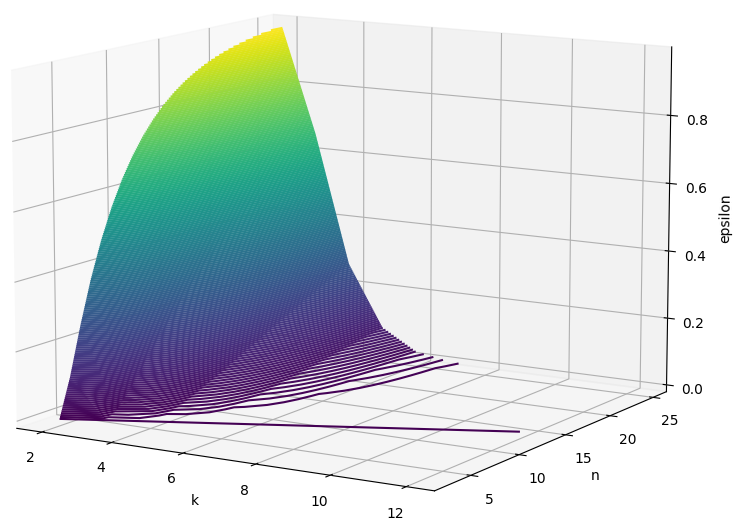
\includegraphics[width=16.5cm]{images/smallNoConsensusBetaOne.png}
    \end{figure*}
    \begin{figure*}
        Probability of not reaching consensus (β = 1) : -log(ε) 
        \centering
        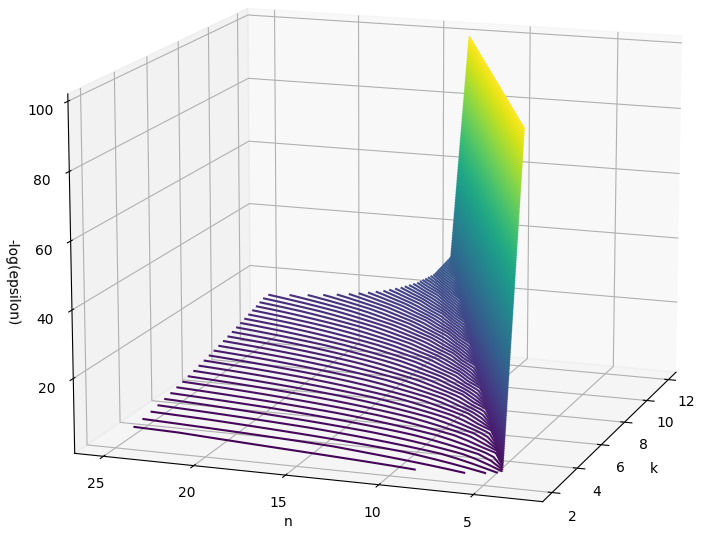
\includegraphics[width=16.5cm]{images/smalllogNoConsensusBetaOne.png}
    \end{figure*}
    \begin{figure*}
        Probability of not reaching consensus (β = 2) : ε 
        \centering
        \includegraphics[width=16.5cm]{images/smallnoconsensus.png}
    \end{figure*}
    \begin{figure*}
        Probability of not reaching consensus (β = 2) : -log(ε) 
        \centering
        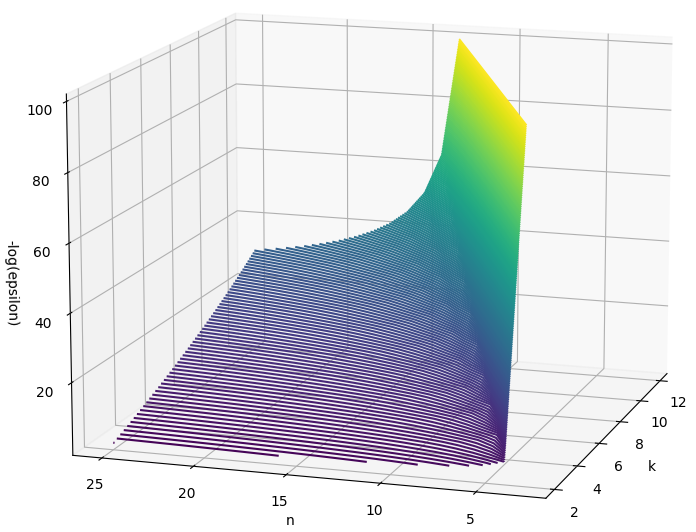
\includegraphics[width=16.5cm]{images/smalllognoconsensus.png}
    \end{figure*}
\end{appendices}
\end{document}
